\section{Introduction}
The field of \textit{artificial intelligence} as been extremely popular over recent years, due to the wide range of applications the technology has developed with the help of modern computer hardware. \textit{Machine learning algorithms} are capable of outperforming humans at a variety of different tasks, while being faster and significantly cheaper to operate. Possible applications for these algorithms include self-driving vehicles, computer-aided interpretation of medical imagery, stock market analysis and robotics. However, despite their impeccable performance, current artificially intelligent programs have a common drawback, which is their inability to generalize to other tasks. Each algorithm is developed by human experts specifically to solve a single problem and is hence referred to as \textit{artificial narrow intelligence}. A program capable of learning many different tasks, similarly to a human, is called \textit{artificial general intelligence} (\textit{AGI}), and developing such a program is the holy grail of artificial intelligence research.

Learning systems can be subdivided into three categories, which are \textit{supervised learning}, \textit{reinforcement learning} and \textit{unsupervised learning}. In supervised learning, the learner is presented with examples of inputs together with the desired outputs, and must adopt a mapping that generalizes to previously unseen inputs, providing useful outputs. For some problems, no examples that include their respective solutions exist, preventing the use of supervised learning. Consider the movement of a bipedal robot. Giving a sufficient amount of training examples on how to walk for a variety of different scenarios to a learner would require us to already have a solution to the problem we are trying to solve. It is, however, relatively trivial to judge the performance of said walker. For example, falling over is easy to detect and clearly undesirable, whereas a forwards movement should be encouraged. Learning only based on this feedback is called reinforcement learning. Finally, unsupervised learning is used for data in which neither a perfect solution nor a rating (as in the former categories) is available. These algorithms try to structure data by finding hidden patterns or similarities, which may, for instance, be used in data visualizations.

While supervised learning is widely applicable and is even considered somewhat solved by some people, reinforcement learning is still in its infancy. This is not due to a lack of use cases however. Robots, for example, often require learning algorithms, as pre-written movement sequences and rules are usually worthless outside of a factory setting. Despite remarkable strides being made in recent times, with reinforcement learning algorithms playing complex board and video games at superhuman level, \textit{sample efficiency}, that is, the effectiveness with which the algorithm learns from few training examples, continues to be an issue. Sample efficiency is especially critical in the field of robotics, as real world training is costly and throttled by physical limitations, and simulations are computationally expensive and inaccurate.

Reinforcement learning algorithms are further classified into two groups. There are \textit{model-free} algortihms, which can be viewed as an algorithm behaving instinctively, and \textit{model-based} algorithms, which plan their next moves ahead of time. The latter is arguably more human-like, and has the added benefit of being comparatively sample efficient. Furthermore, it is clear why a robot interacting with an environment, for example by catching a ball, would benefit from anticipating the behavior of other objects within its vicinity, especially when considering the delay between sensory information arriving and its motors being actuated.

The \textit{MuZero Algorithm} \cite{muzero} has made recent breakthroughs by becoming the new state-of-the-art model-based reinforcement learning algorithm. It outperforms its predecessors in a variety of tasks, while simultaneously being very sample efficient. This makes it appear to be a general purpose algorithm and an excellent candidate for our experiments involving robot grasping (see figure \ref{fig:cube_stacking}).
\begin{figure}[ht]
    \centering
    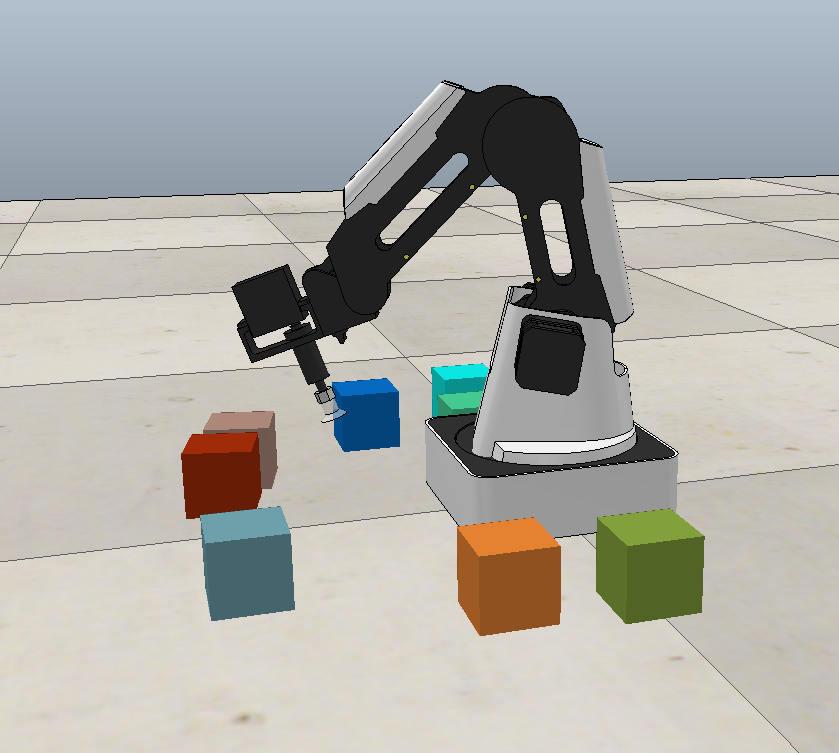
\includegraphics[width=0.5\textwidth]{assets/cube_stacking.png}
    \caption{A \textit{Dobot} robotic arm being tasked with picking up and stacking simulated cubes in \textit{CoppeliaSim} (\url{https://www.coppeliarobotics.com/}).}
    \label{fig:cube_stacking}
\end{figure}

Unfortunately, upon further investigation, we realized that MuZero performed relatively poorly on our robot experiments and was slow to operate. Contrary to our expectations, older, model-free algorithms such as \textit{A3C} \cite{a3c} delivered significantly better results while being more lightweight and easy to implement. Even in very basic tasks, our own implementation as well as code provided by other researchers produced unsatisfactory benchmarks.

This leads us to believe that MuZero may require team of experts and expensive hardware to reach its full potential. We question some of the design decisions made for MuZero and attempt to make it more approachable.